%
%
%
\subsection{Transonic buffeting over a bicircular airfoil}
\label{transonic_buffeting.subsec}
%
 Starting for about 1976, several experiments were
 carried out on transonic buffeting over bicircular-arc airfoils
 at NASA Ames research center with the intent to provide
 basic data to guide further development of computer codes
 (McDevitt et al. \citeyearNP{McDevitt:1}).
 The wind tunnel used for those experiments was designed for
 this purpose in order to minimize upper and lower wall
 interference effects. The tests were conducted at free-stream
 Reynolds numbers, based on airfoil chord length, ranging from 1
 to 17 million. The test Mach number was varied from near the critical
 value of 0.71 to the highest possible without the airfoil chocking
 the channel.
 McDevitt et al. \citeyear{McDevitt:1} presented unsteady results for
 a biconvex circular-arc airfoil with thickness-chord ratio of 0.18.
 The nominal test Mach for this airfoil is 0.775 and the wind
 tunnel end walls were designed to minimize wall effects for this flow
 condition.
%
%
\begin{figure}[ht]
 \begin{center}
  \begin{tabular}{ccc}
    \subfigure[Time 1]
       {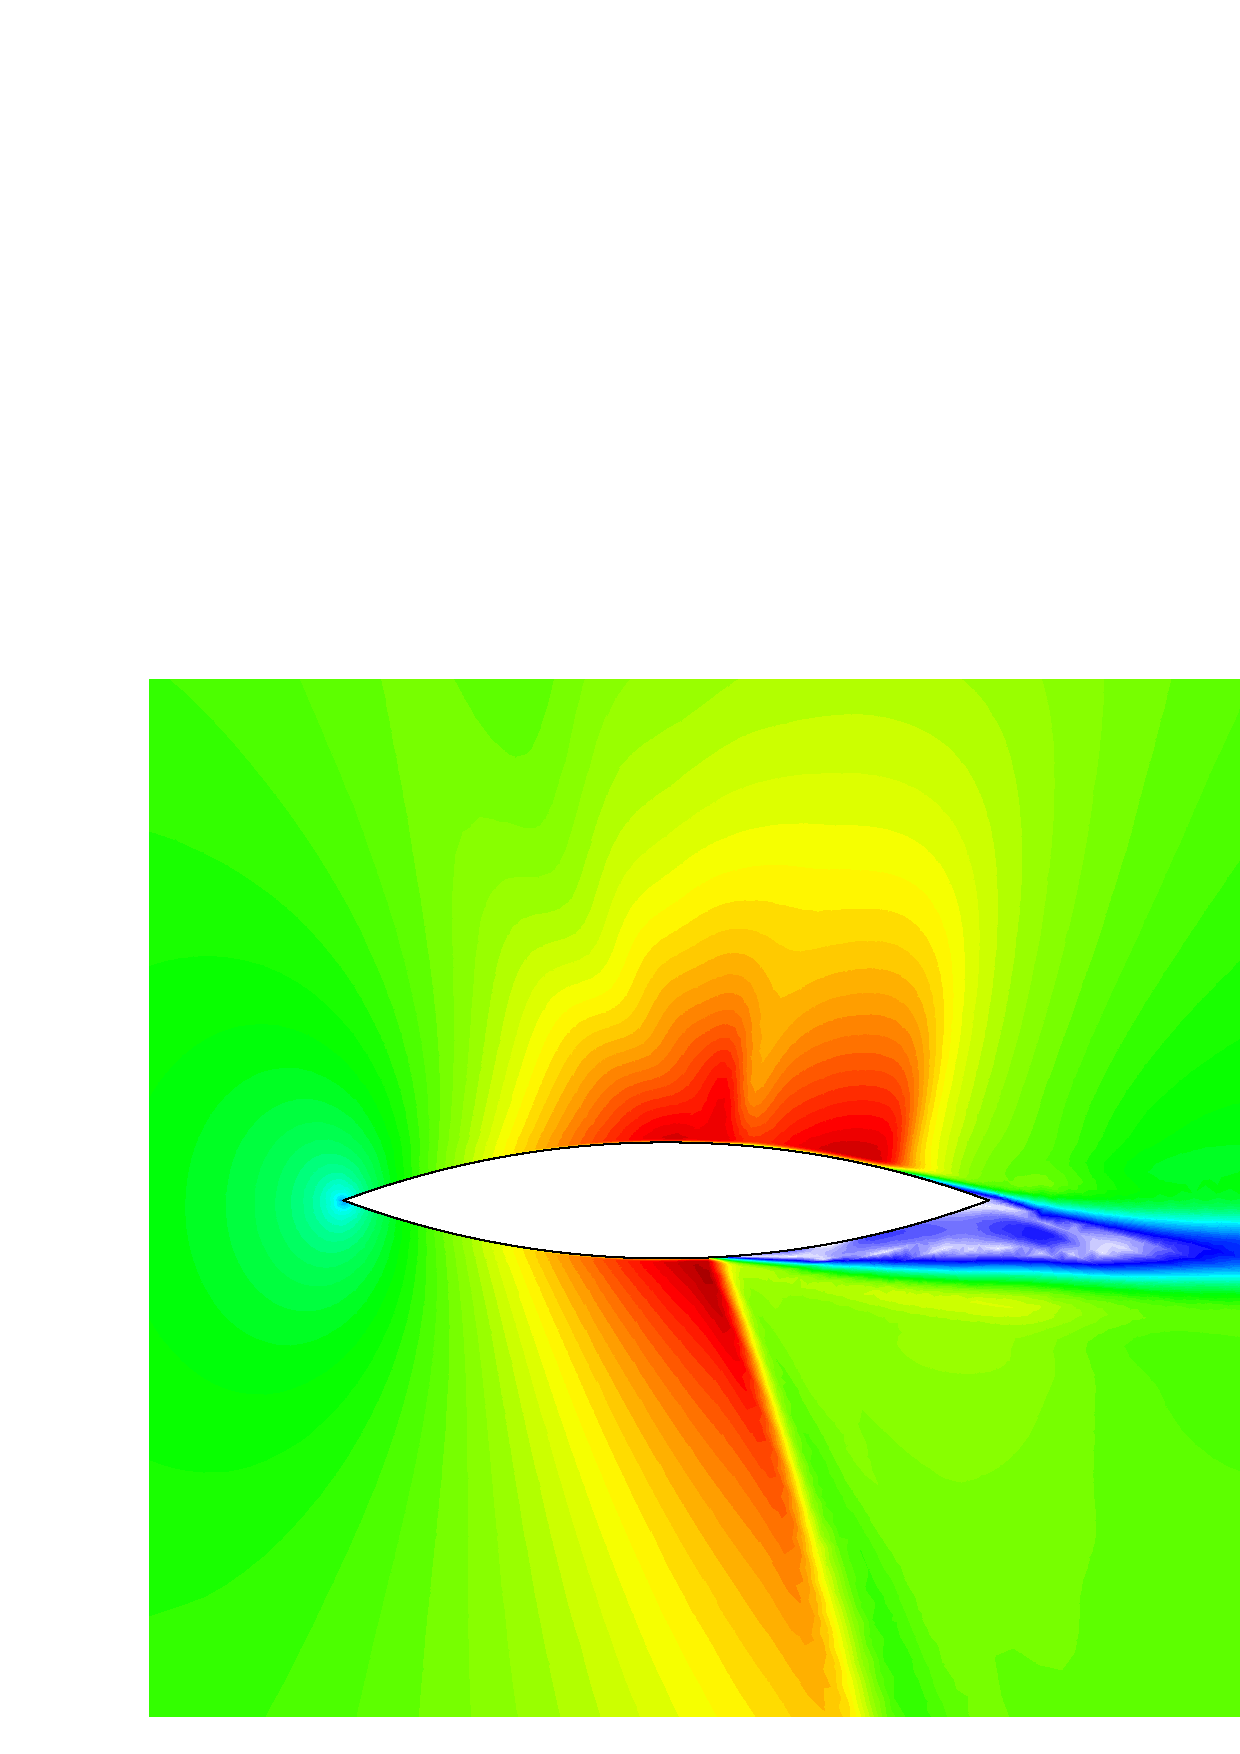
\includegraphics[width=45mm,clip=t]{CHAP_NONLIN/FIGURE/arc1.pdf}}
        &
    \subfigure[Time 2]
       {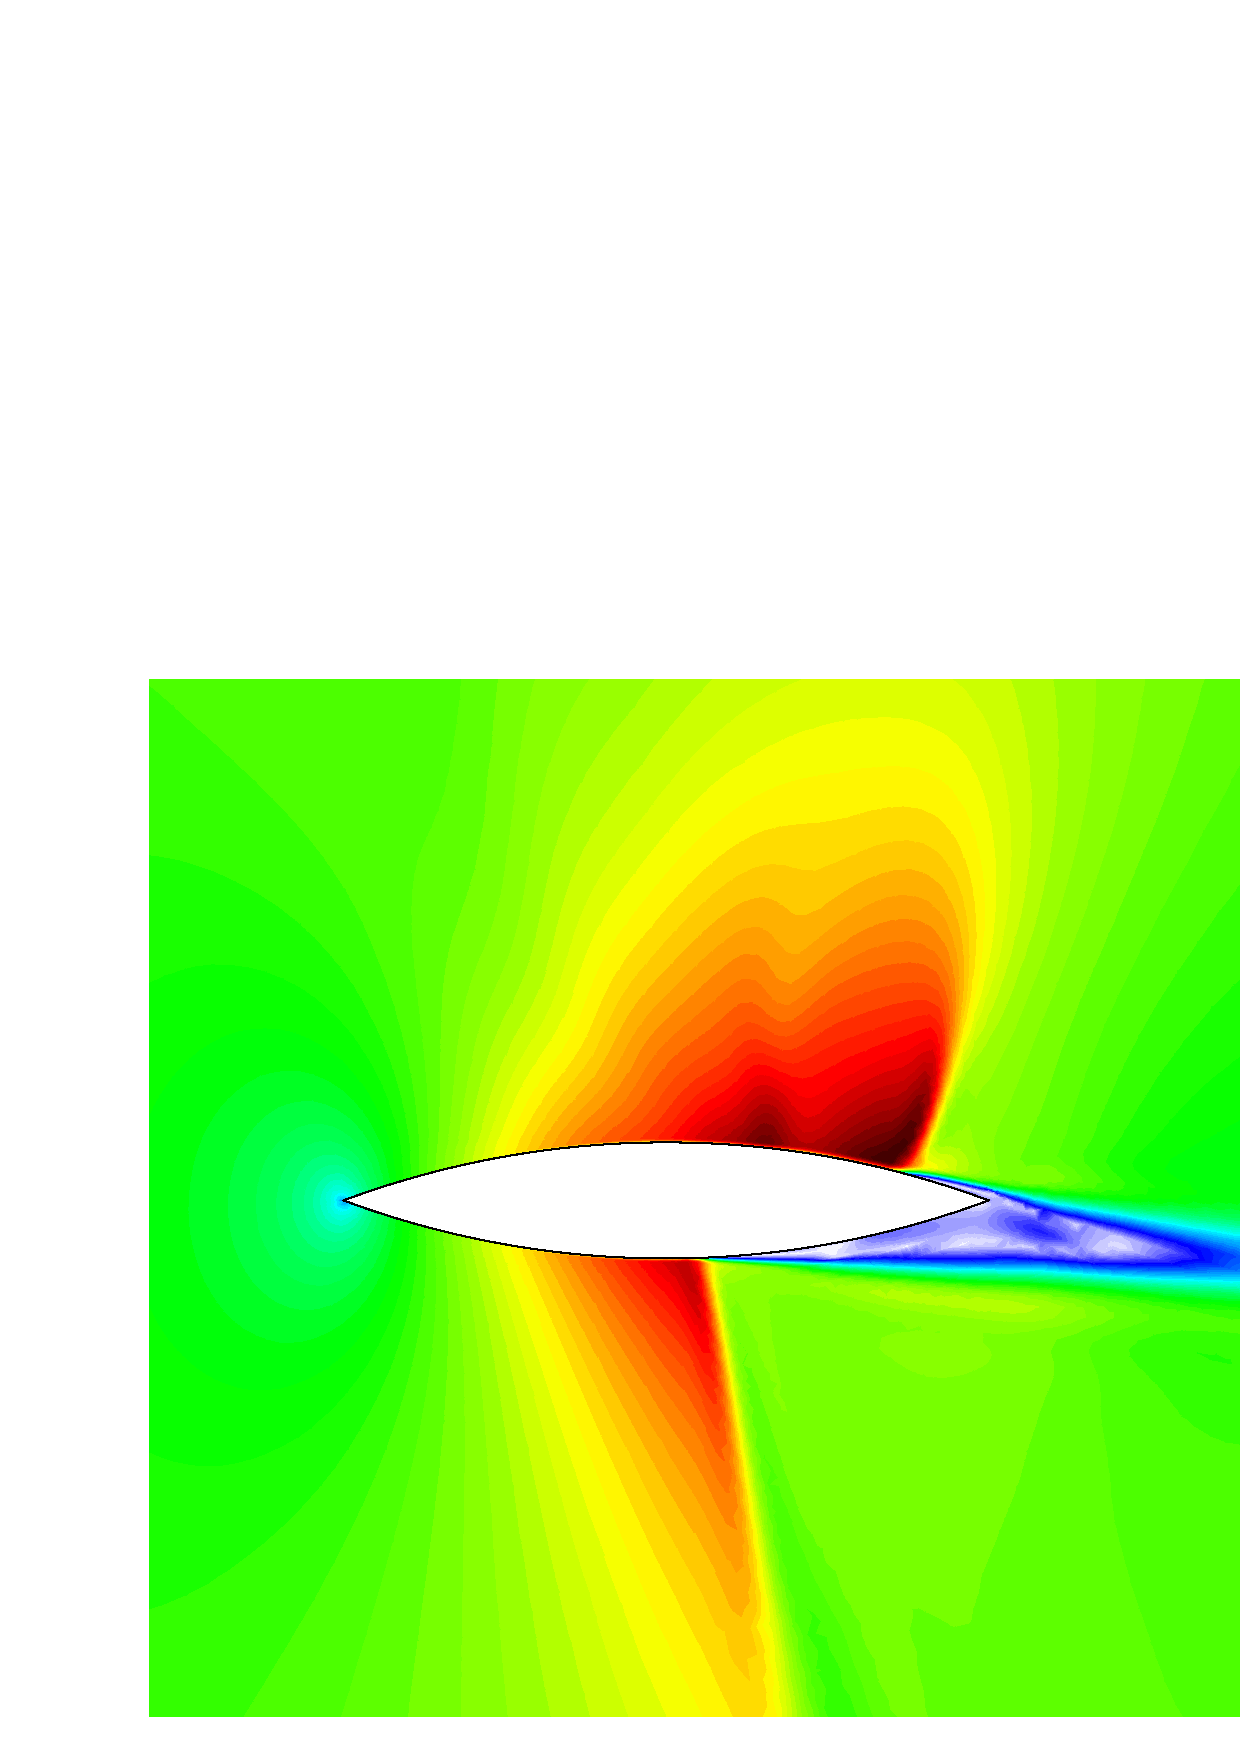
\includegraphics[width=45mm,clip=t]{CHAP_NONLIN/FIGURE/arc2.pdf}}
        &
    \subfigure[Time 3]
       {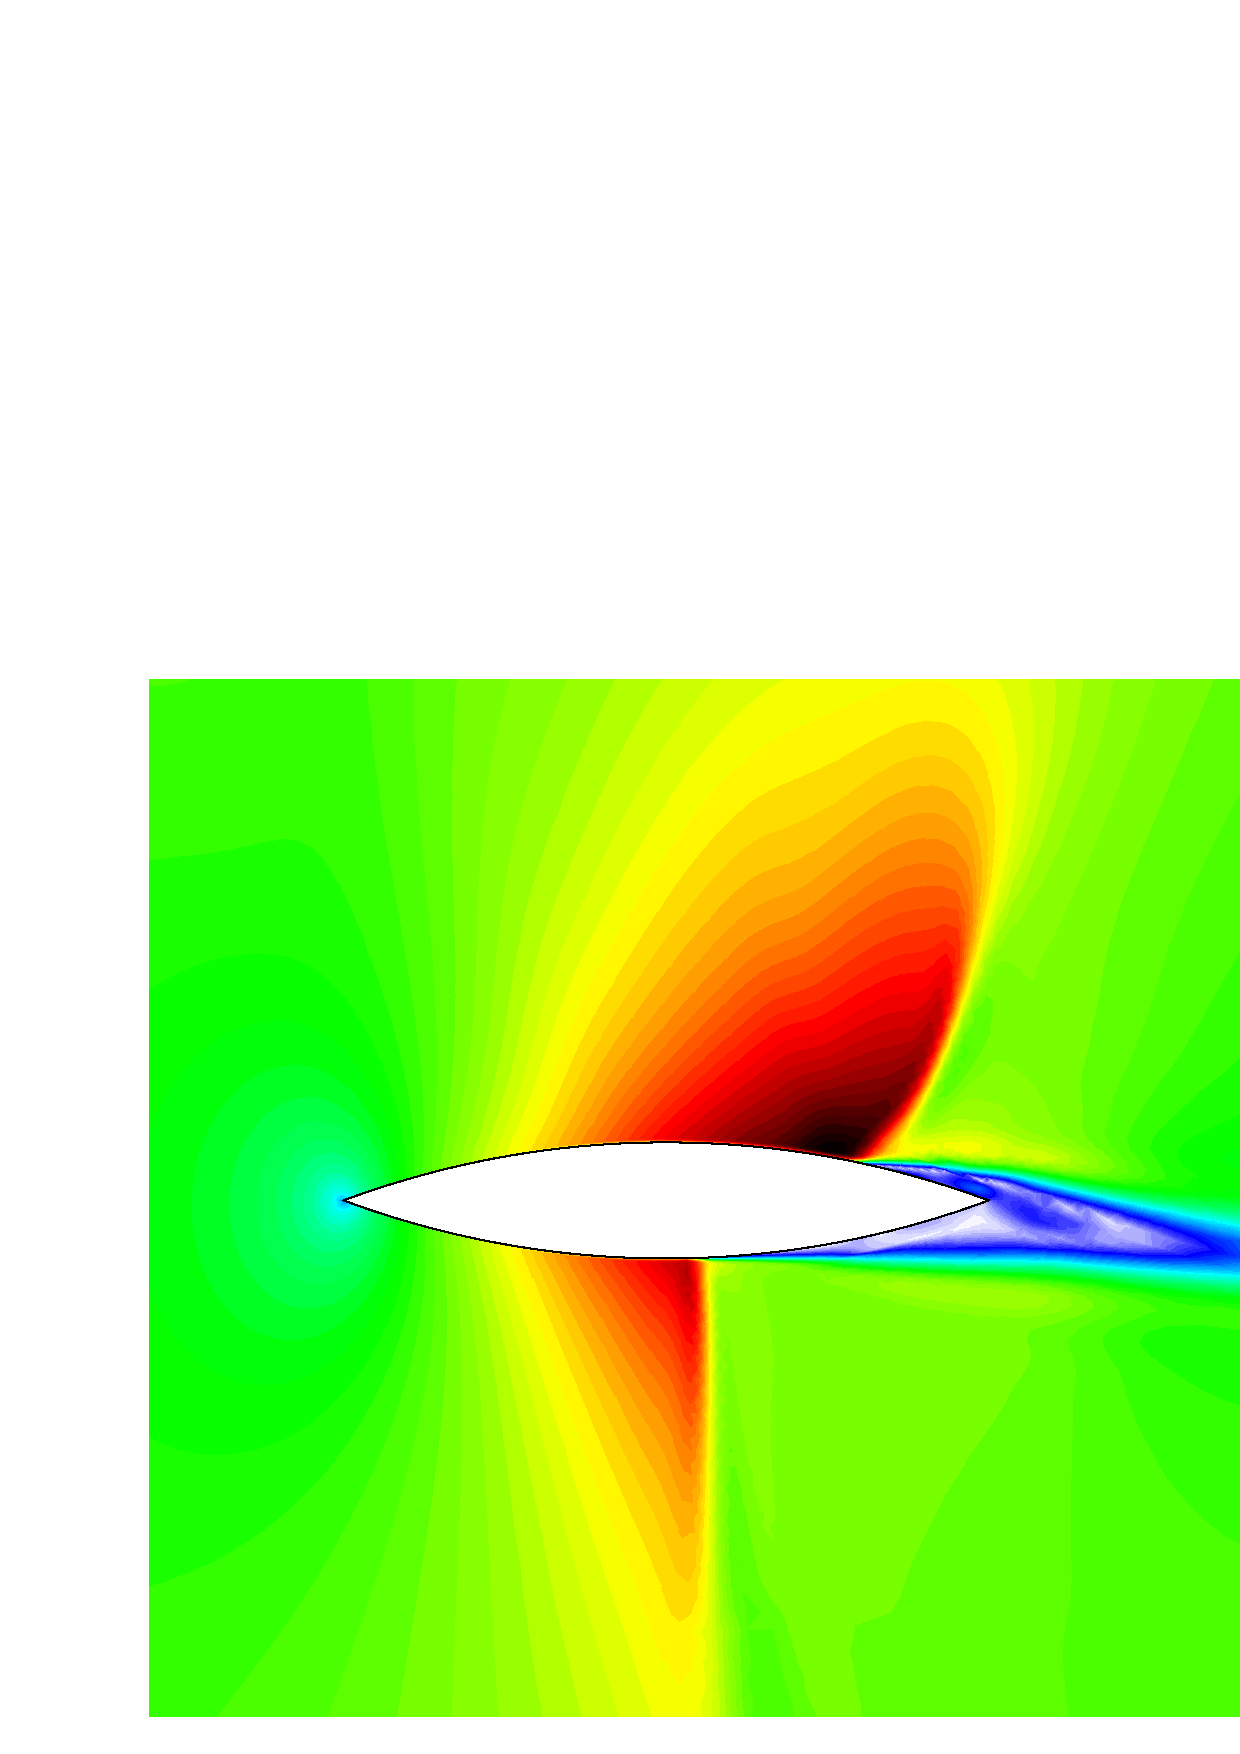
\includegraphics[width=45mm,clip=t]{CHAP_NONLIN/FIGURE/arc3.pdf}}
        \vspace{-4mm}\\
    \subfigure[Time 4]
       {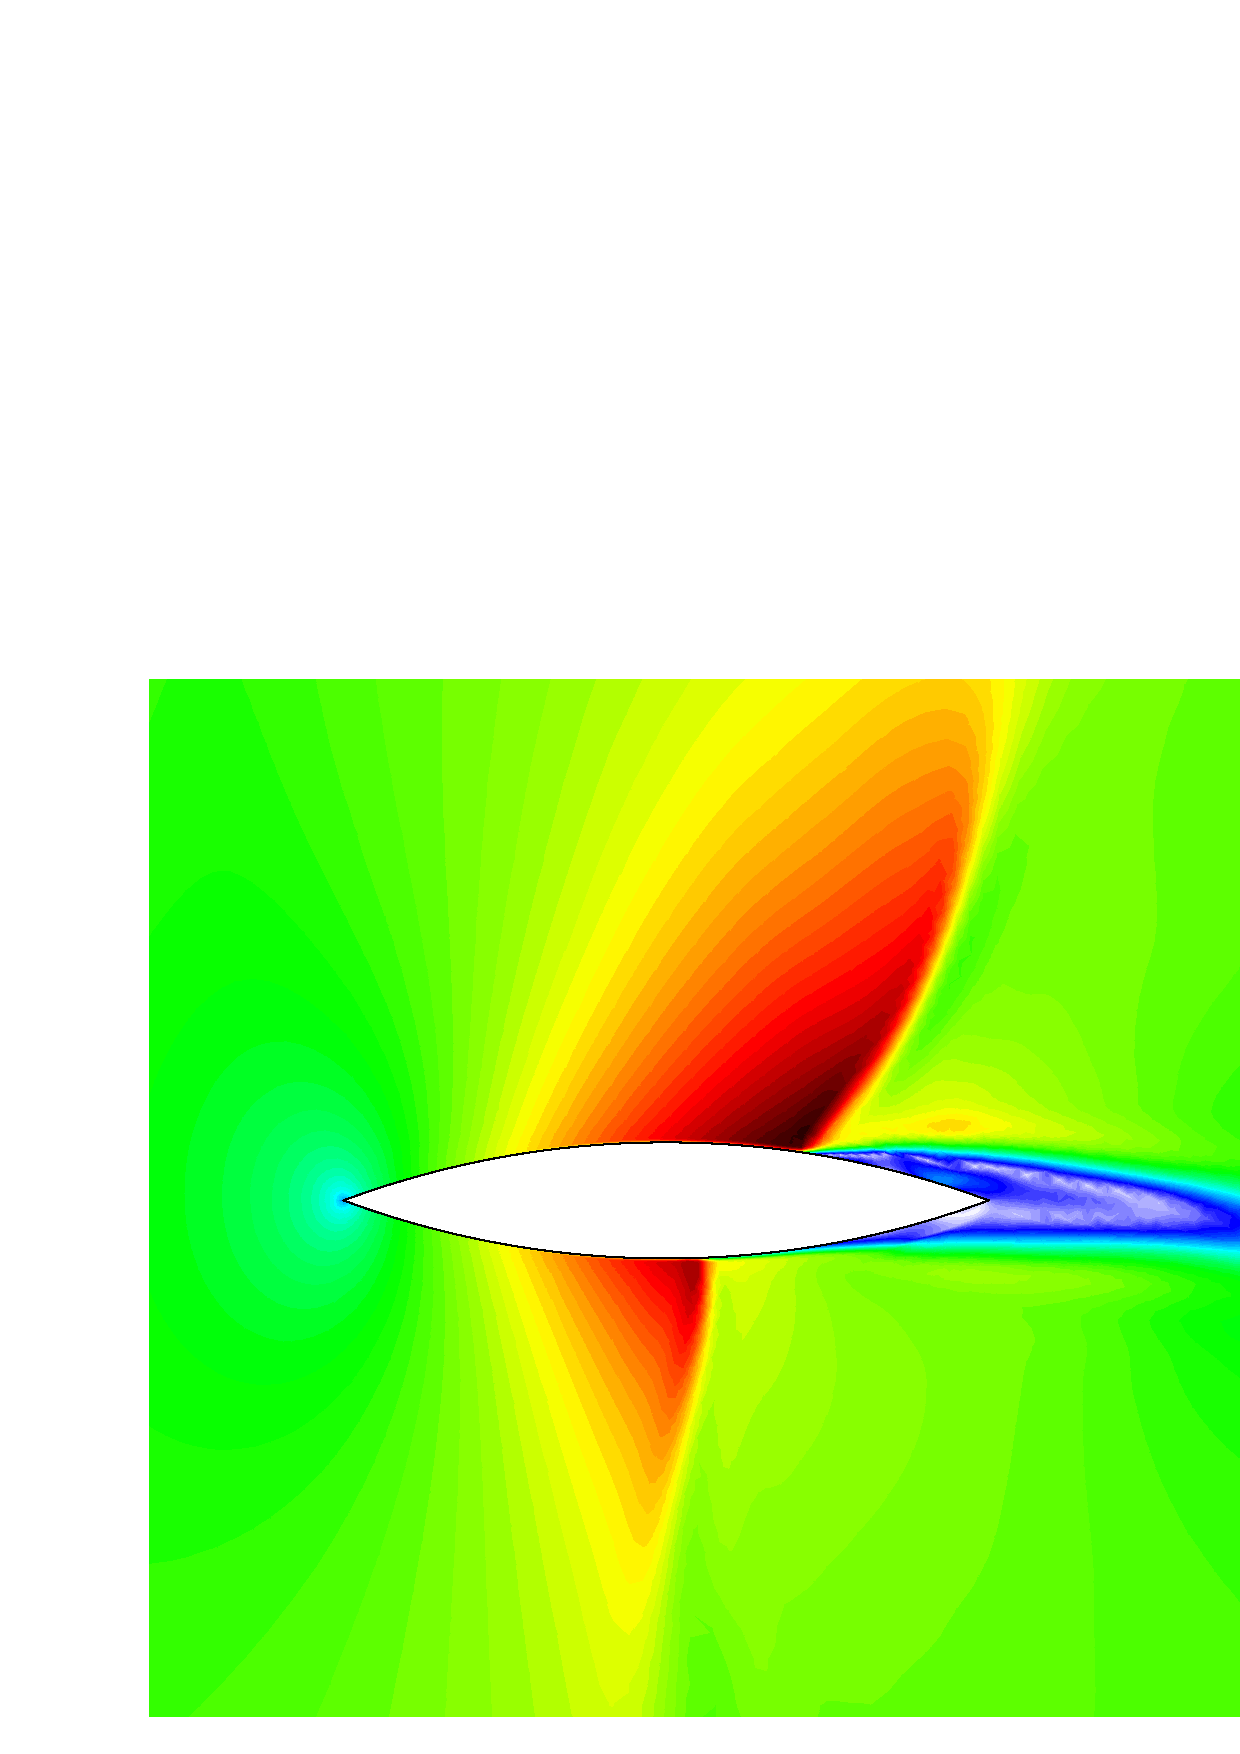
\includegraphics[width=45mm,clip=t]{CHAP_NONLIN/FIGURE/arc4.pdf}}
        &
    \subfigure[Time 5]
       {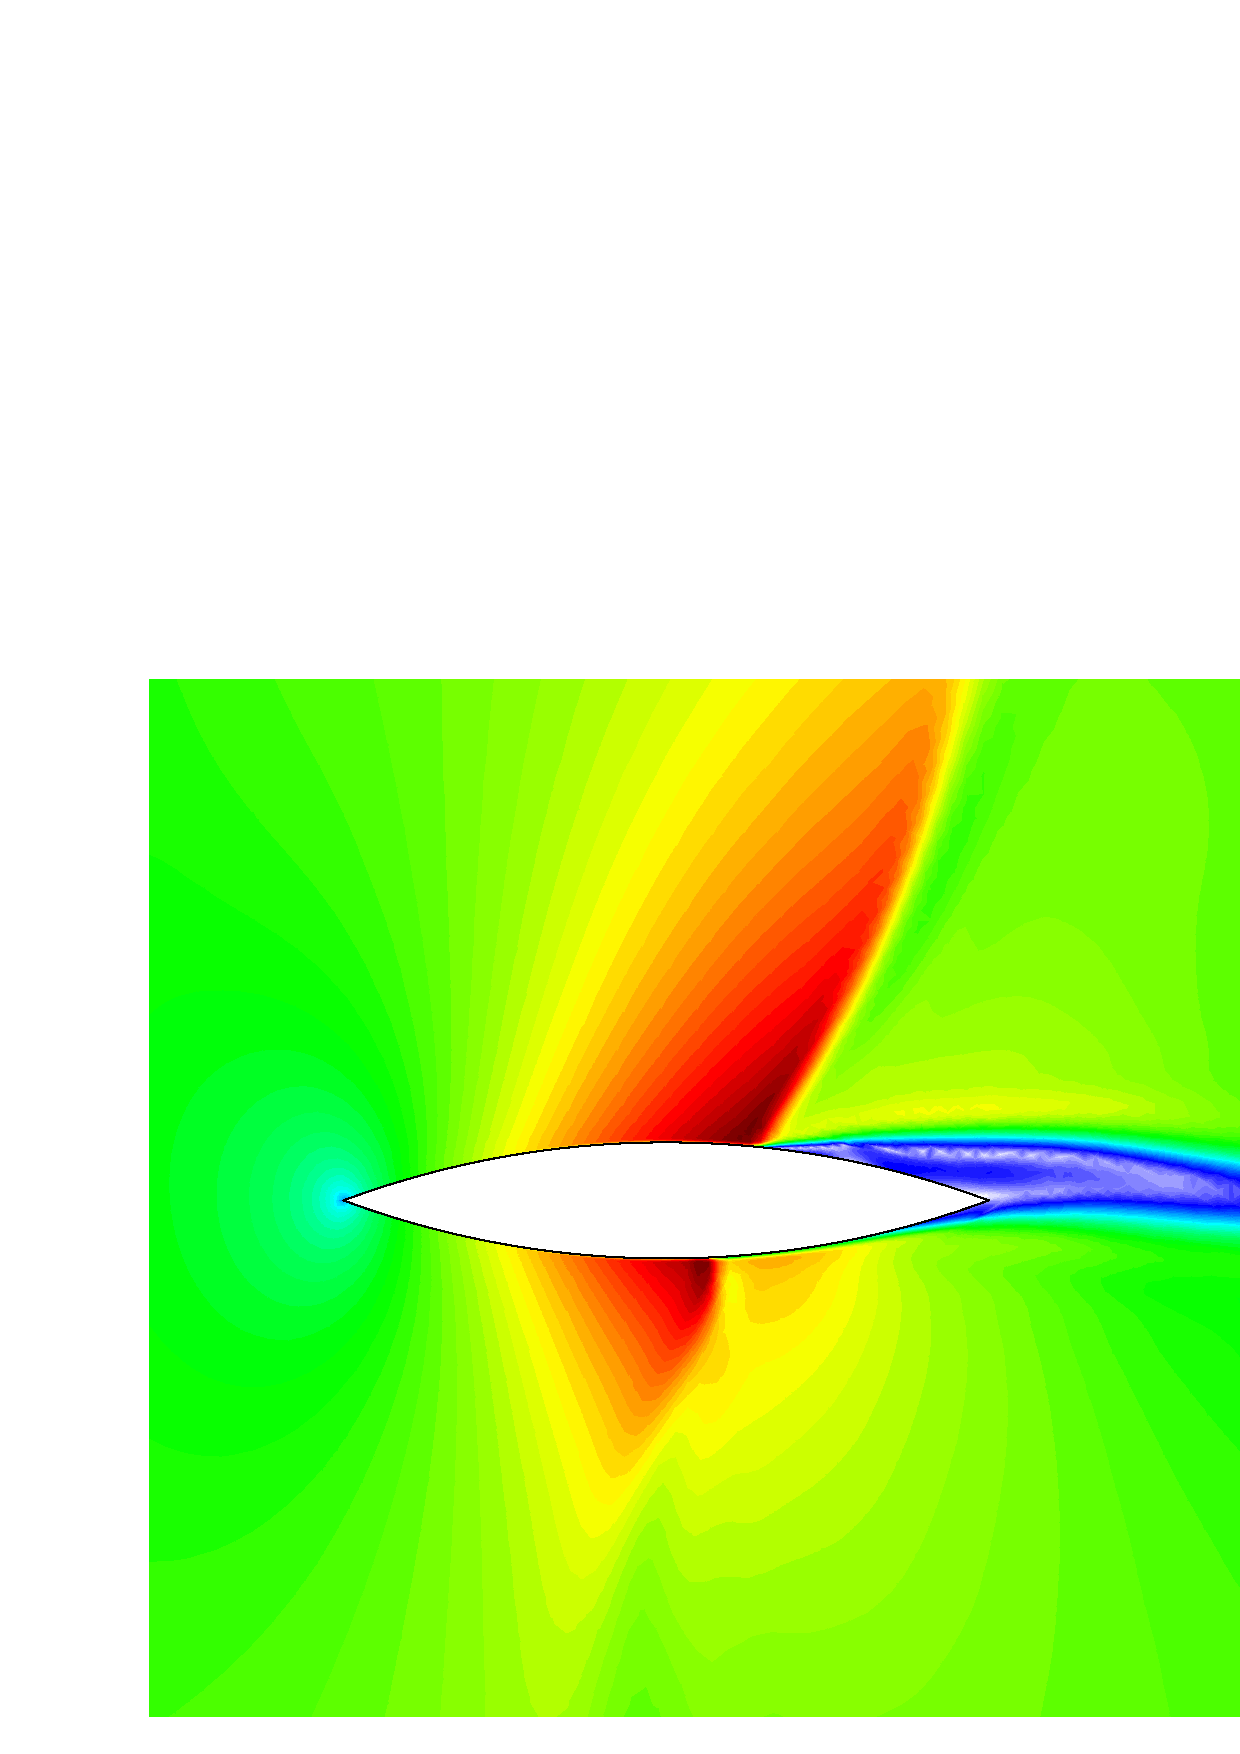
\includegraphics[width=45mm,clip=t]{CHAP_NONLIN/FIGURE/arc5.pdf}}
        &
    \subfigure[Time 6]
       {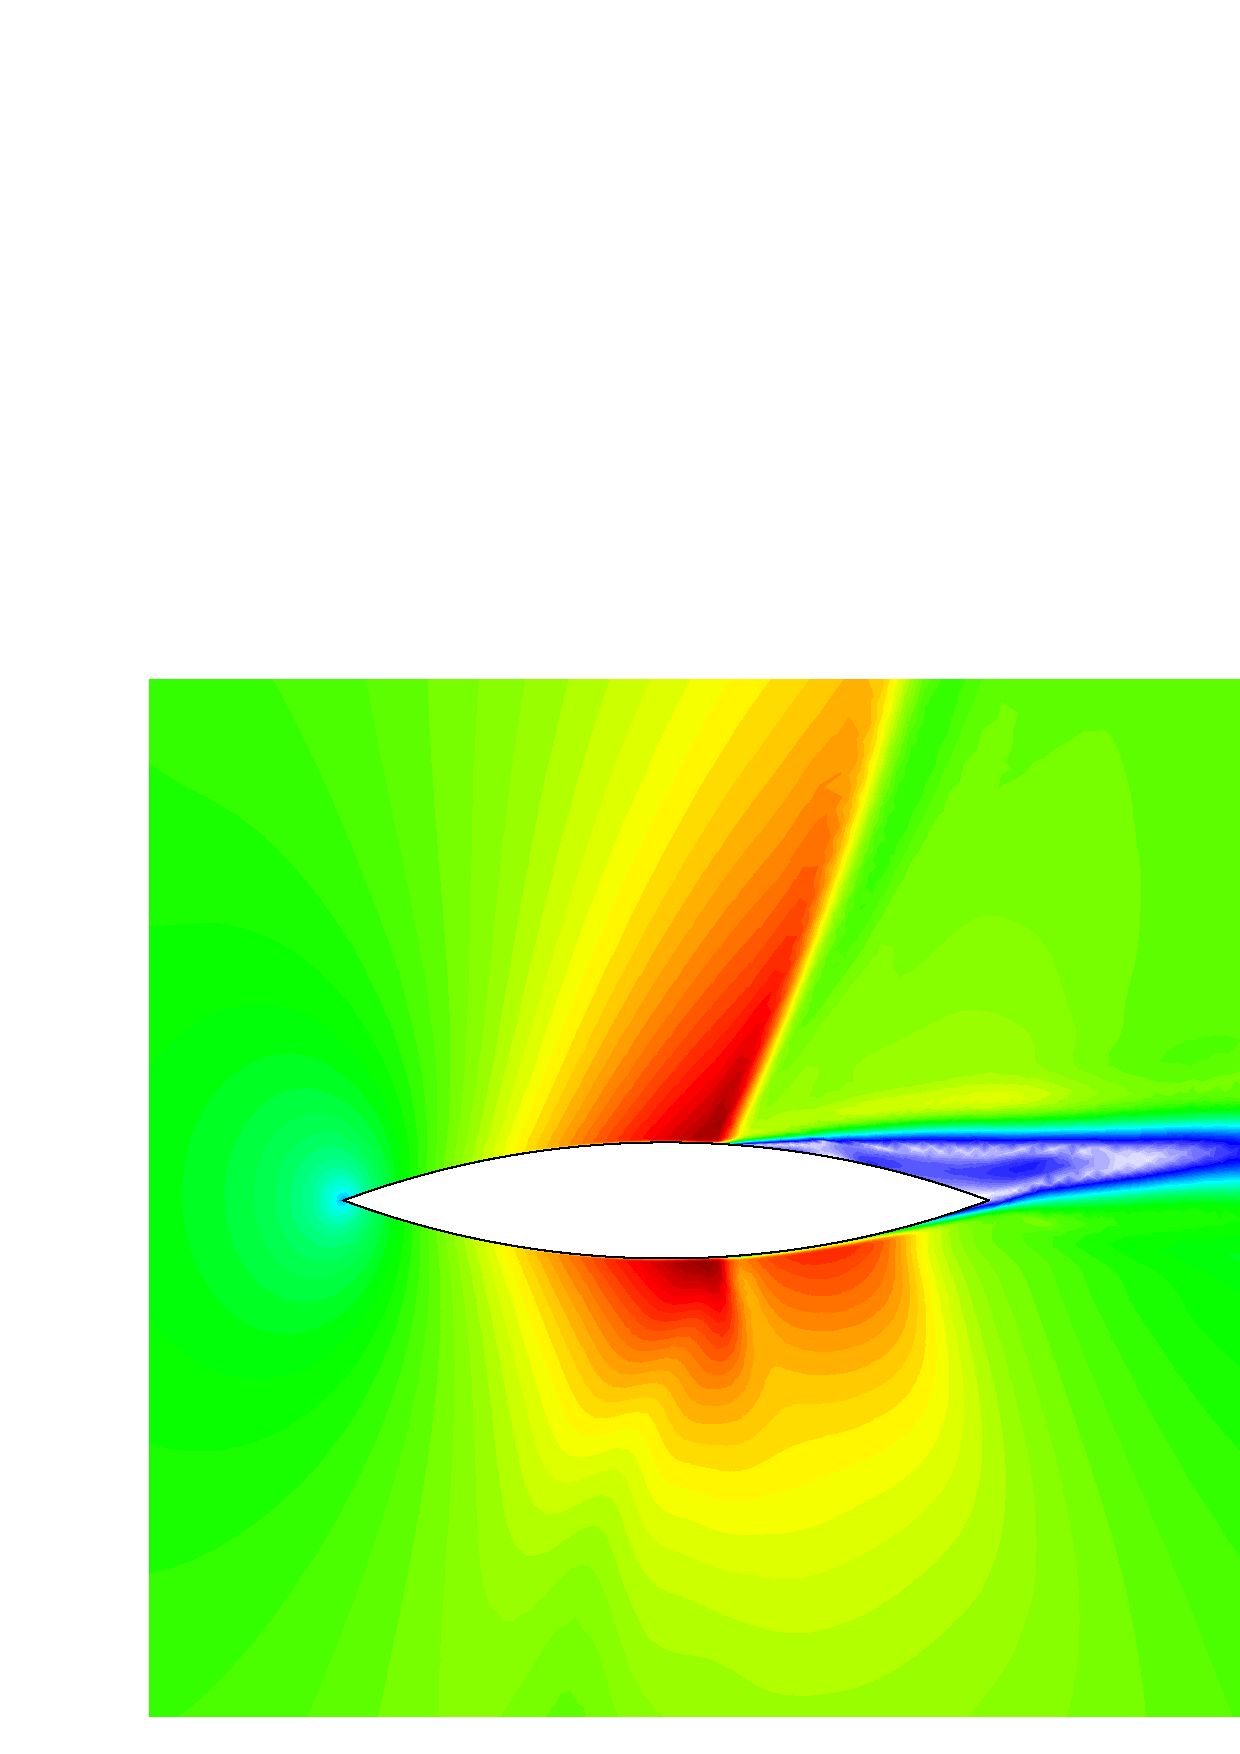
\includegraphics[width=45mm,clip=t]{CHAP_NONLIN/FIGURE/arc6.pdf}}
        \vspace{-4mm}\\
    \subfigure[Time 7]
       {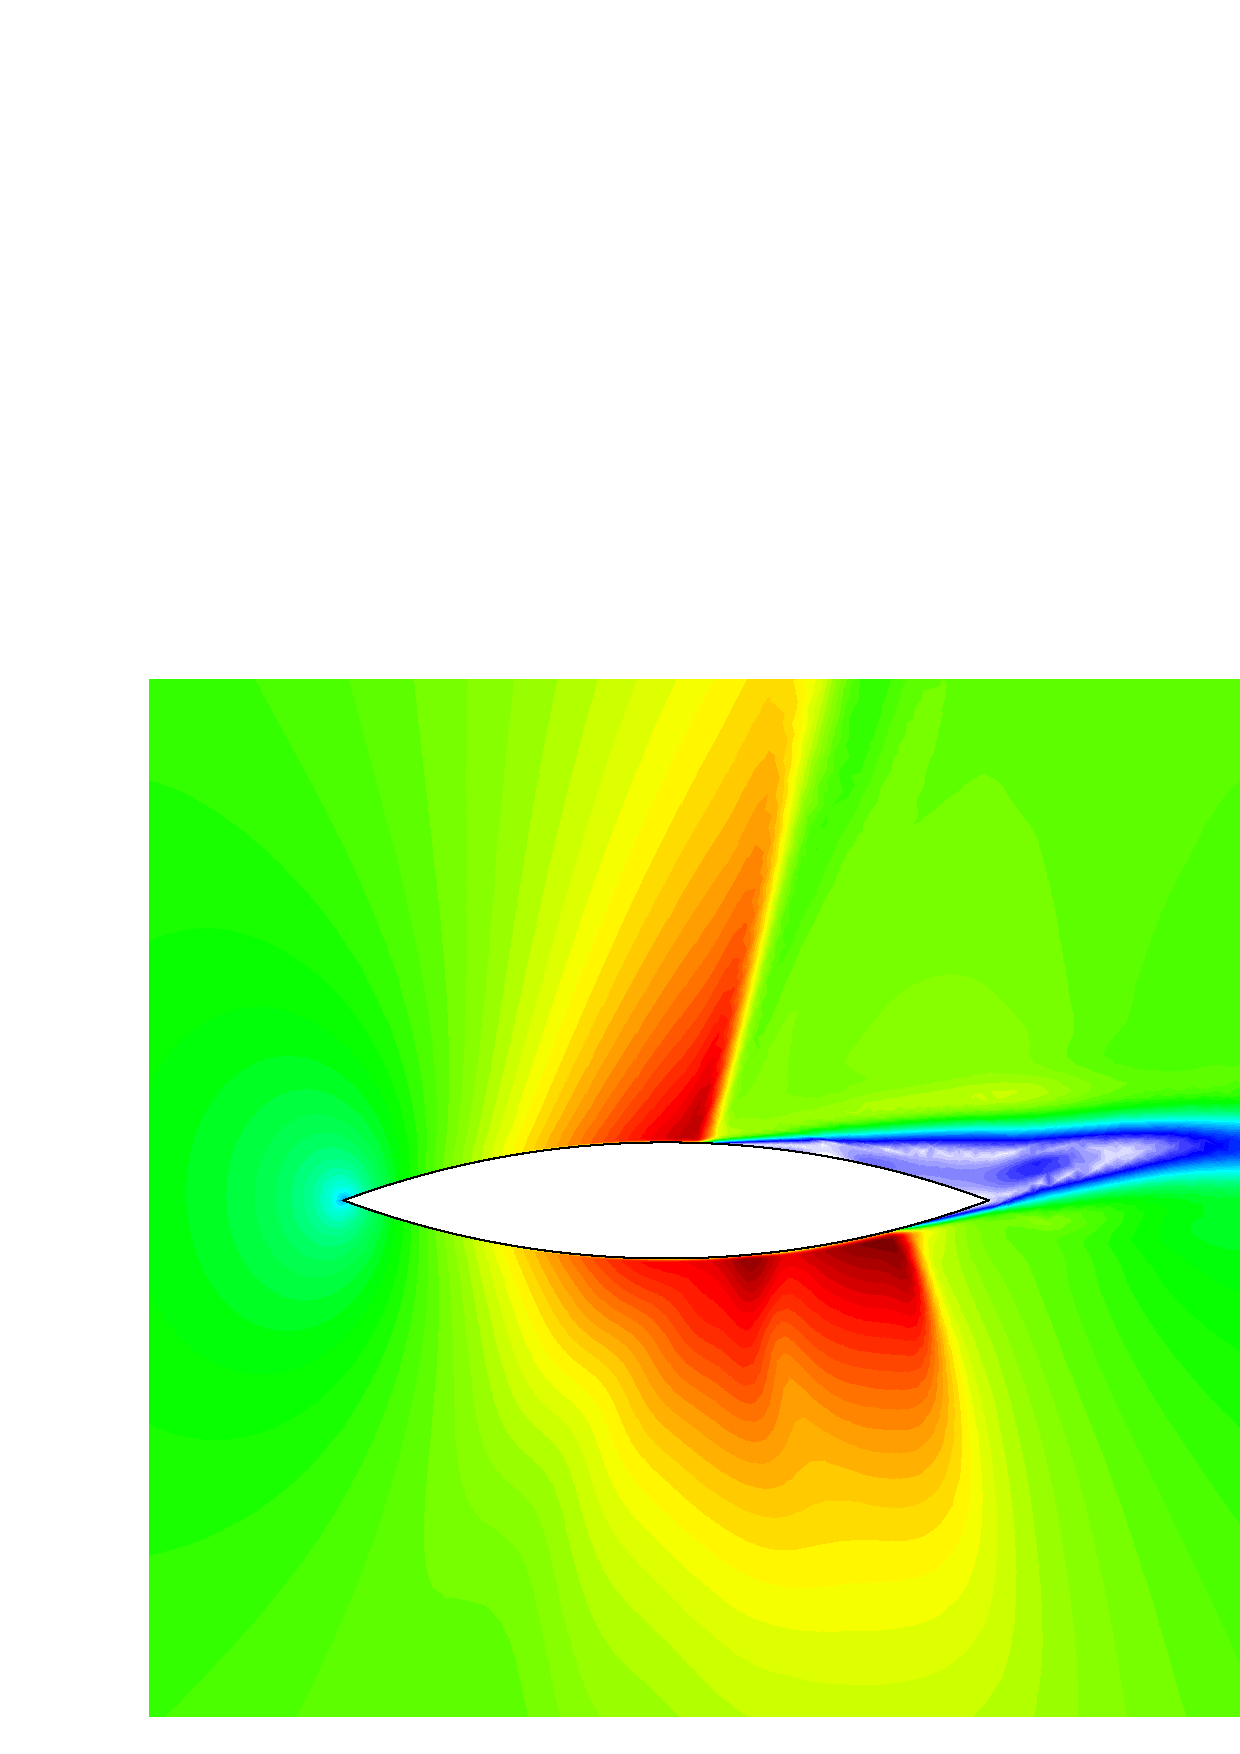
\includegraphics[width=45mm,clip=t]{CHAP_NONLIN/FIGURE/arc7.pdf}}
        &
    \subfigure[Time 8]
       {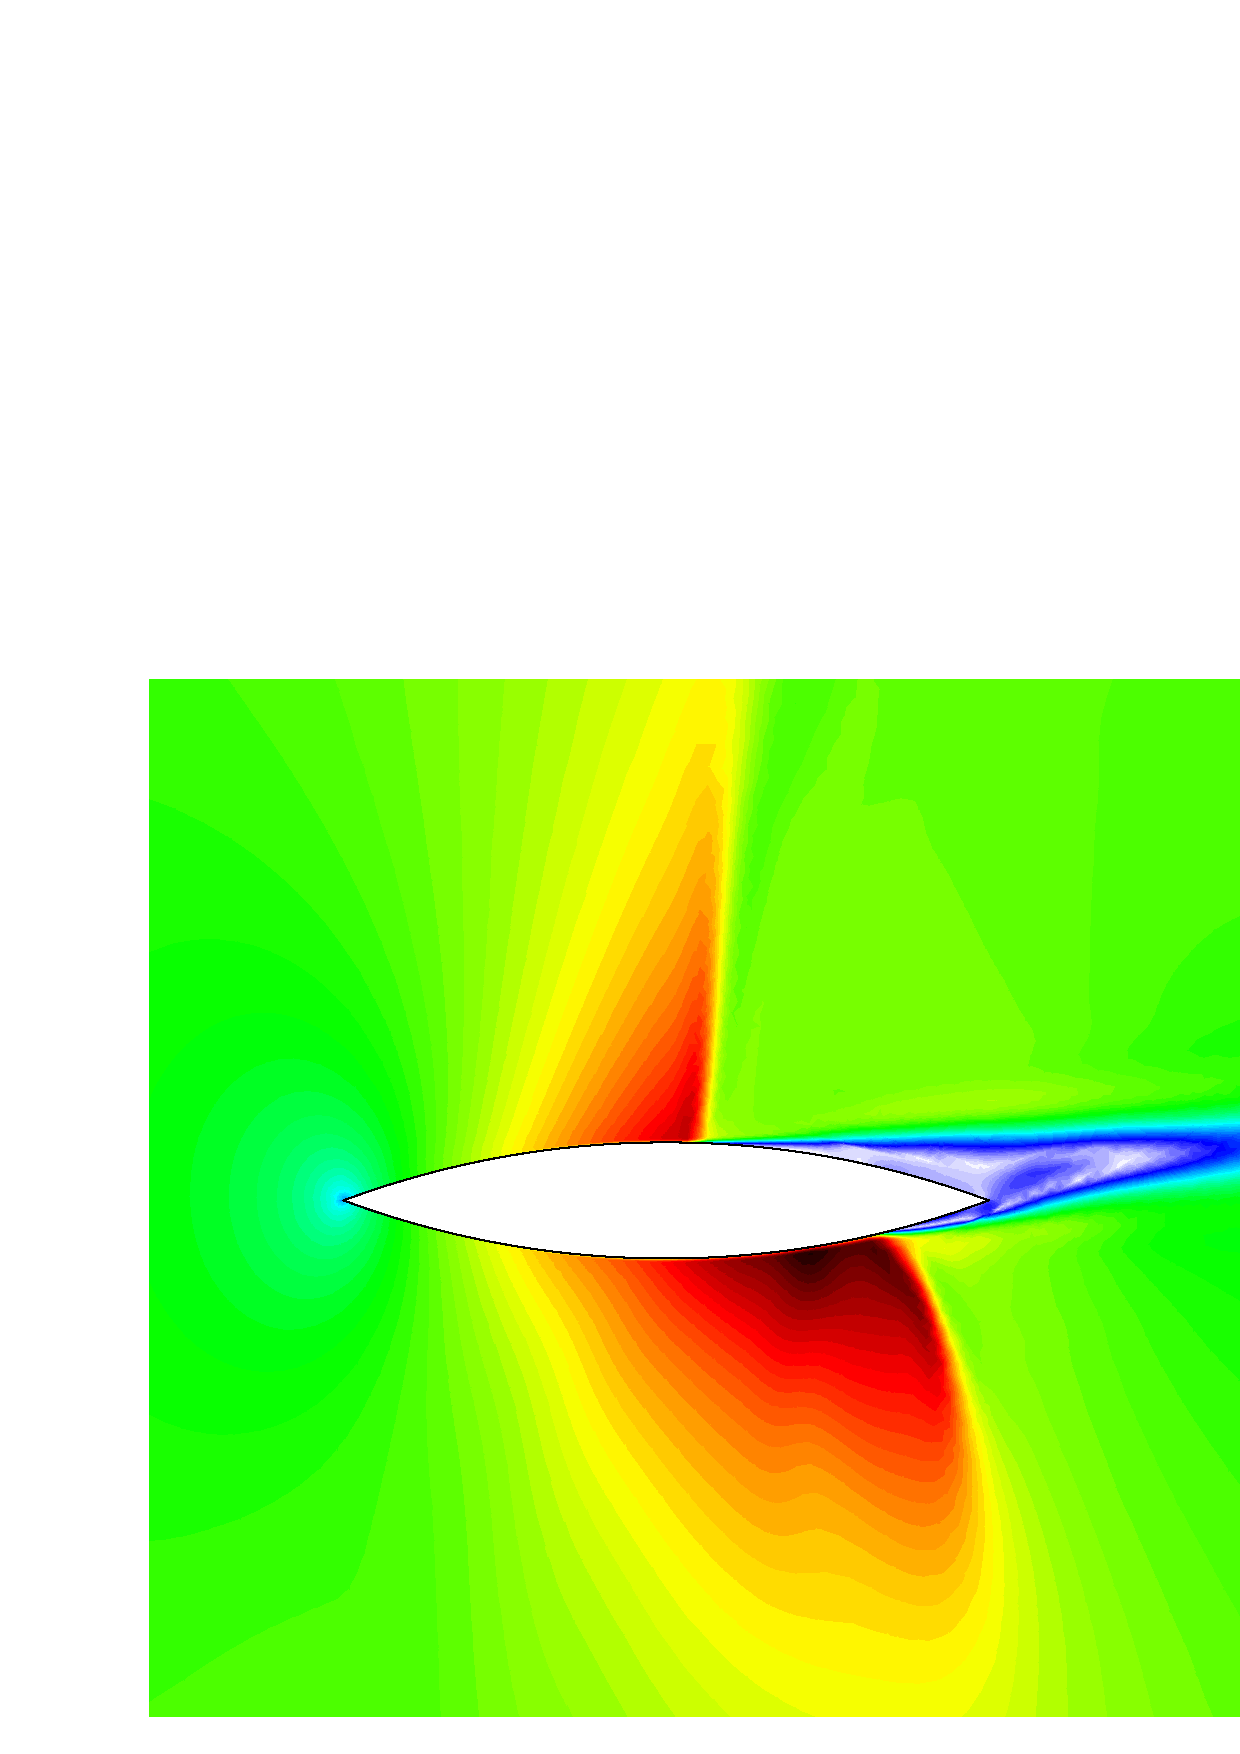
\includegraphics[width=45mm,clip=t]{CHAP_NONLIN/FIGURE/arc8.pdf}}
        &
    \subfigure[Time 9]
       {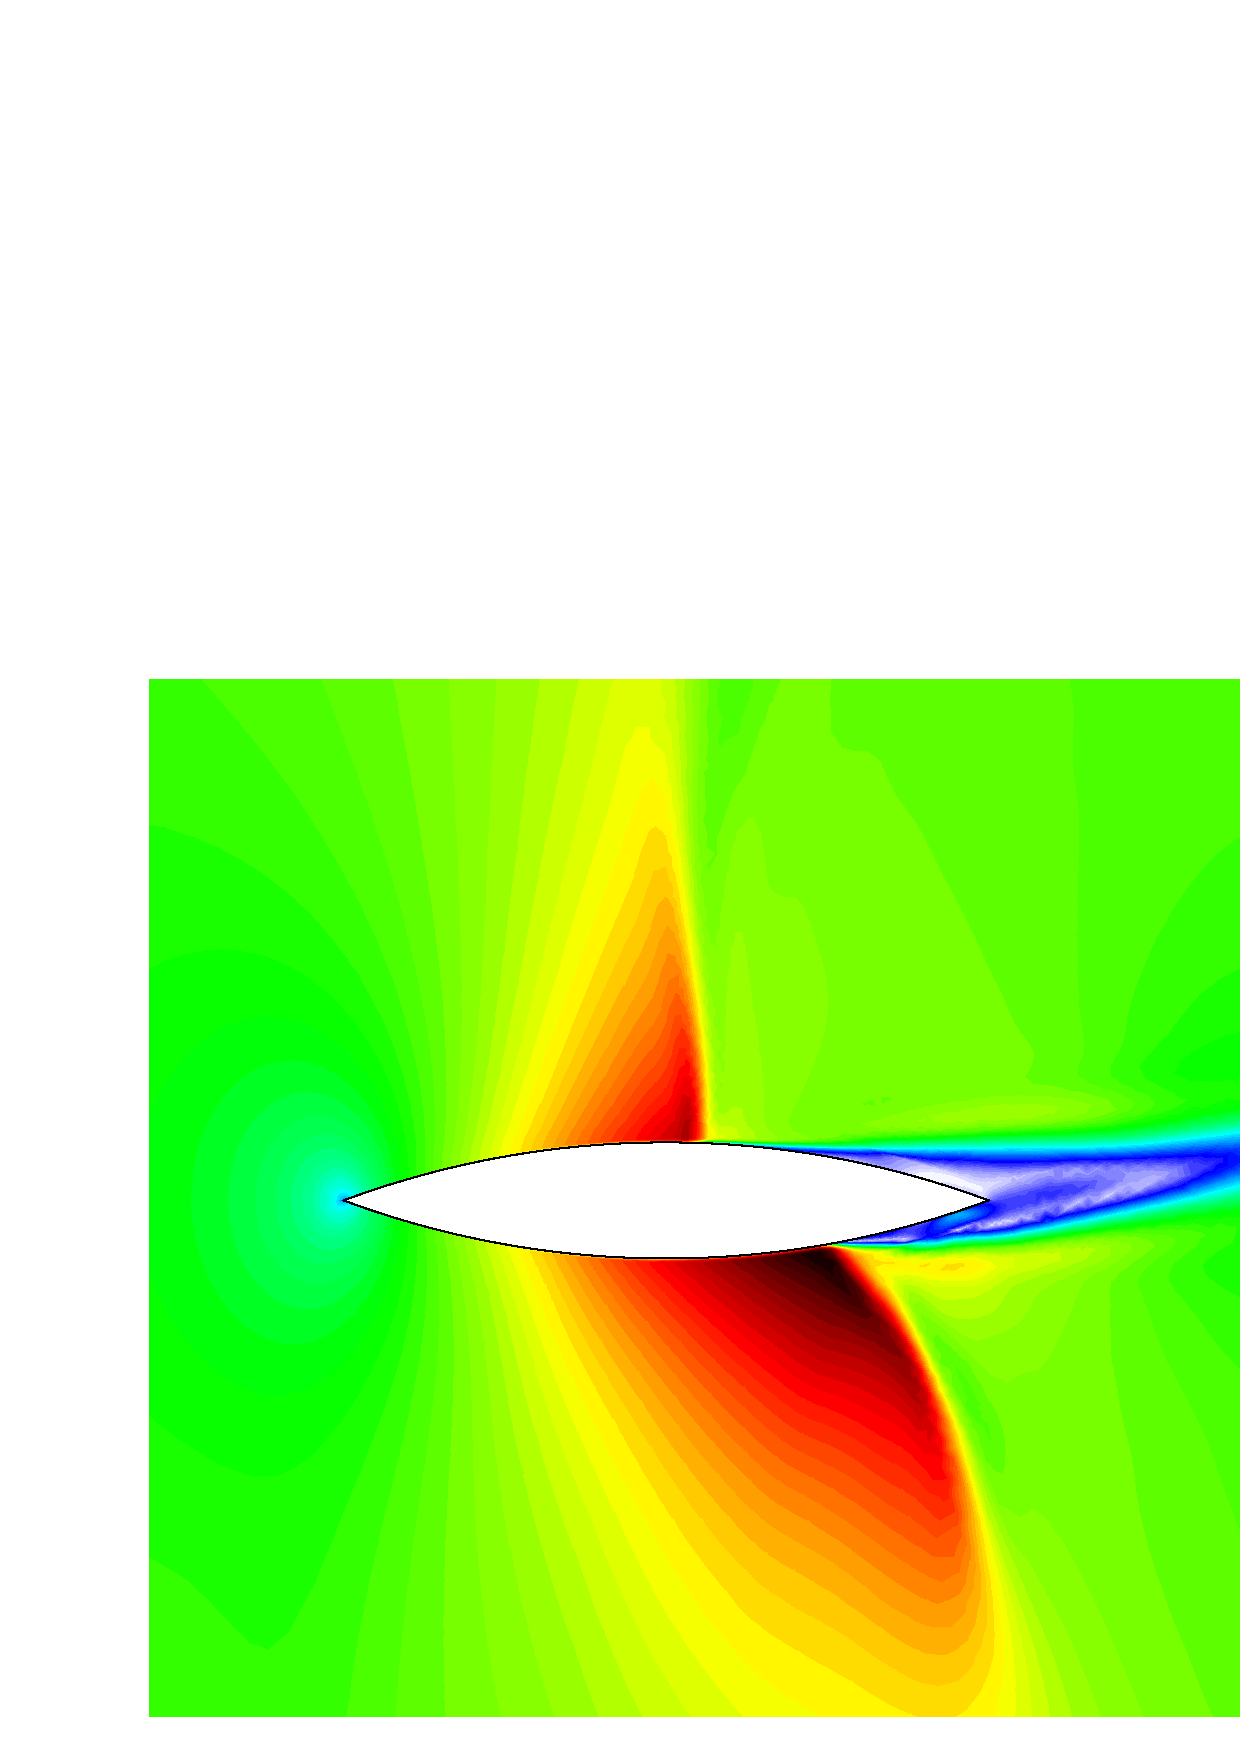
\includegraphics[width=45mm,clip=t]{CHAP_NONLIN/FIGURE/arc9.pdf}}
        \vspace{-4mm}\\
    \subfigure[Time 10]
       {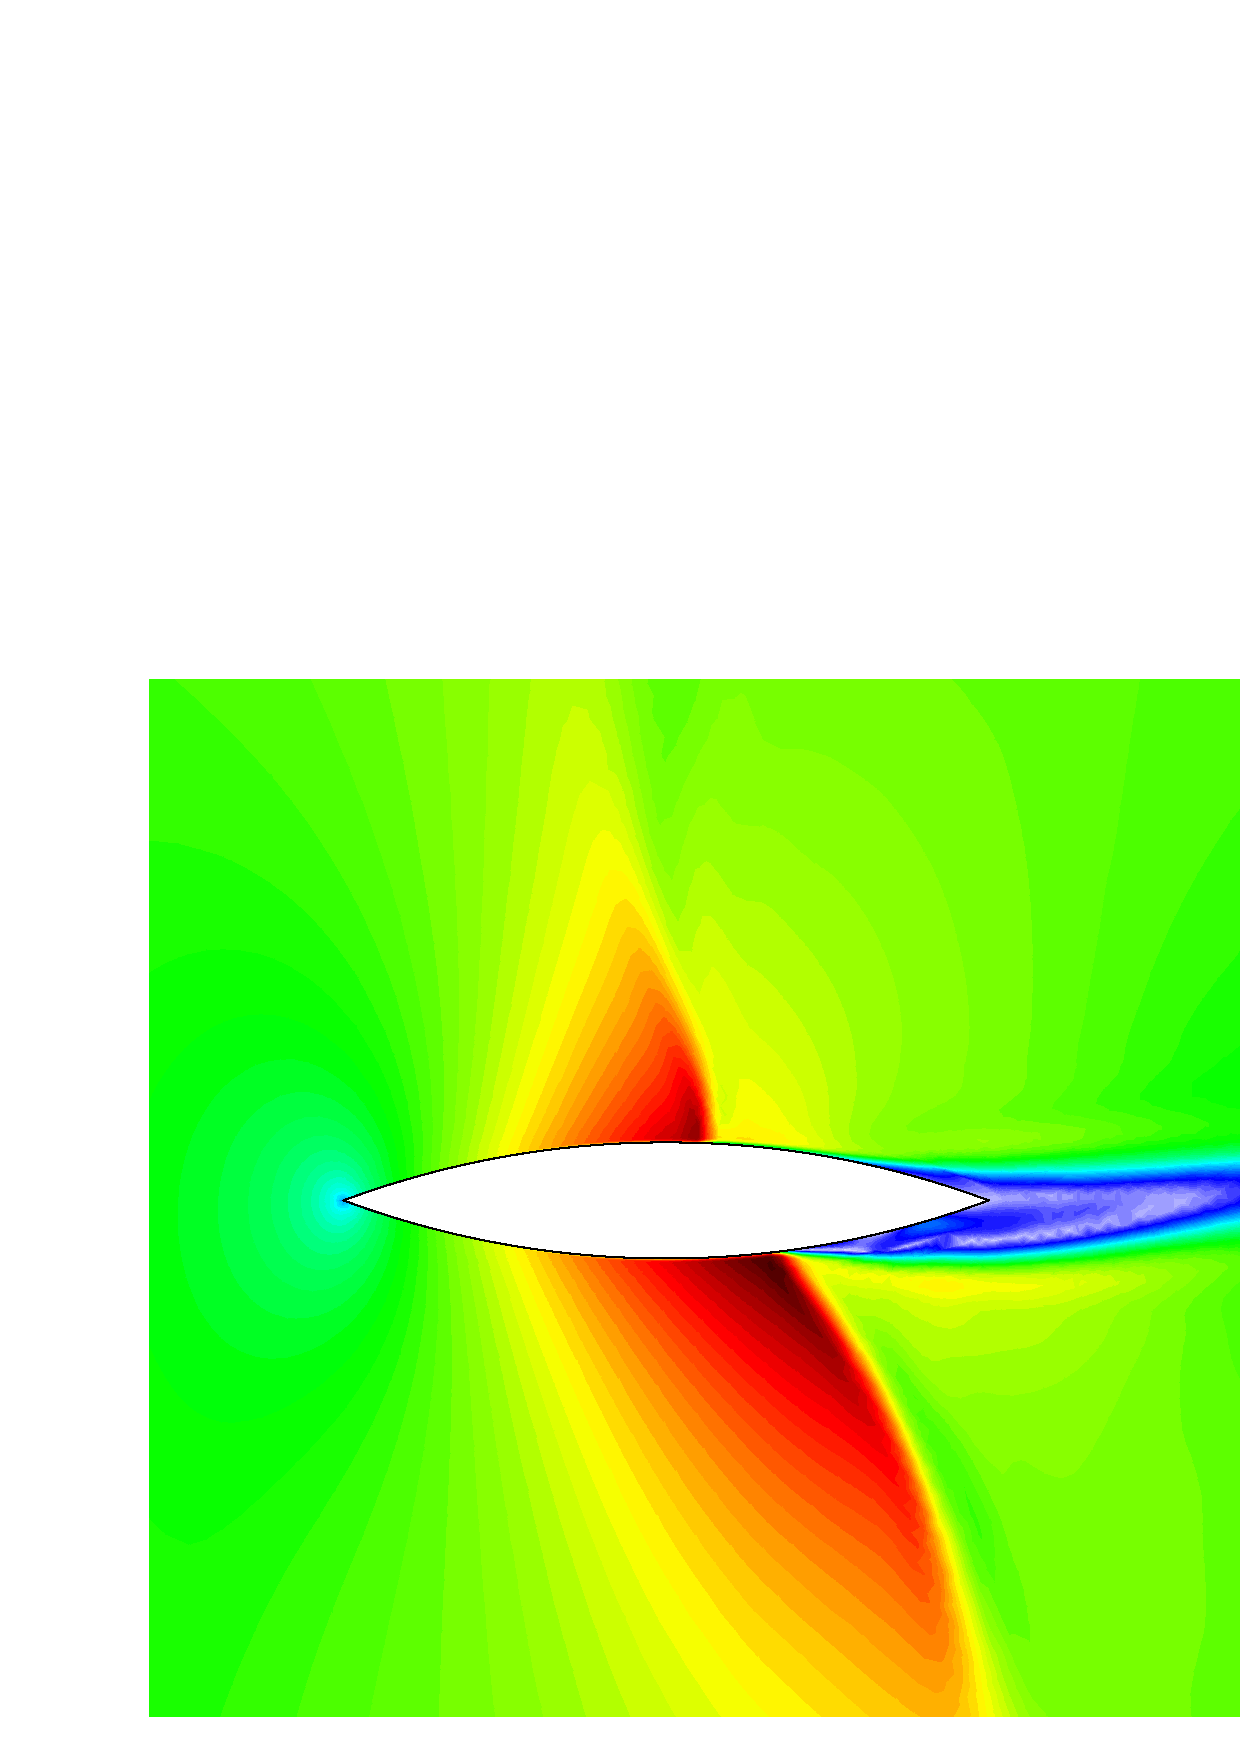
\includegraphics[width=45mm,clip=t]{CHAP_NONLIN/FIGURE/arc10.pdf}}
        &
    \subfigure[Time 11]
       {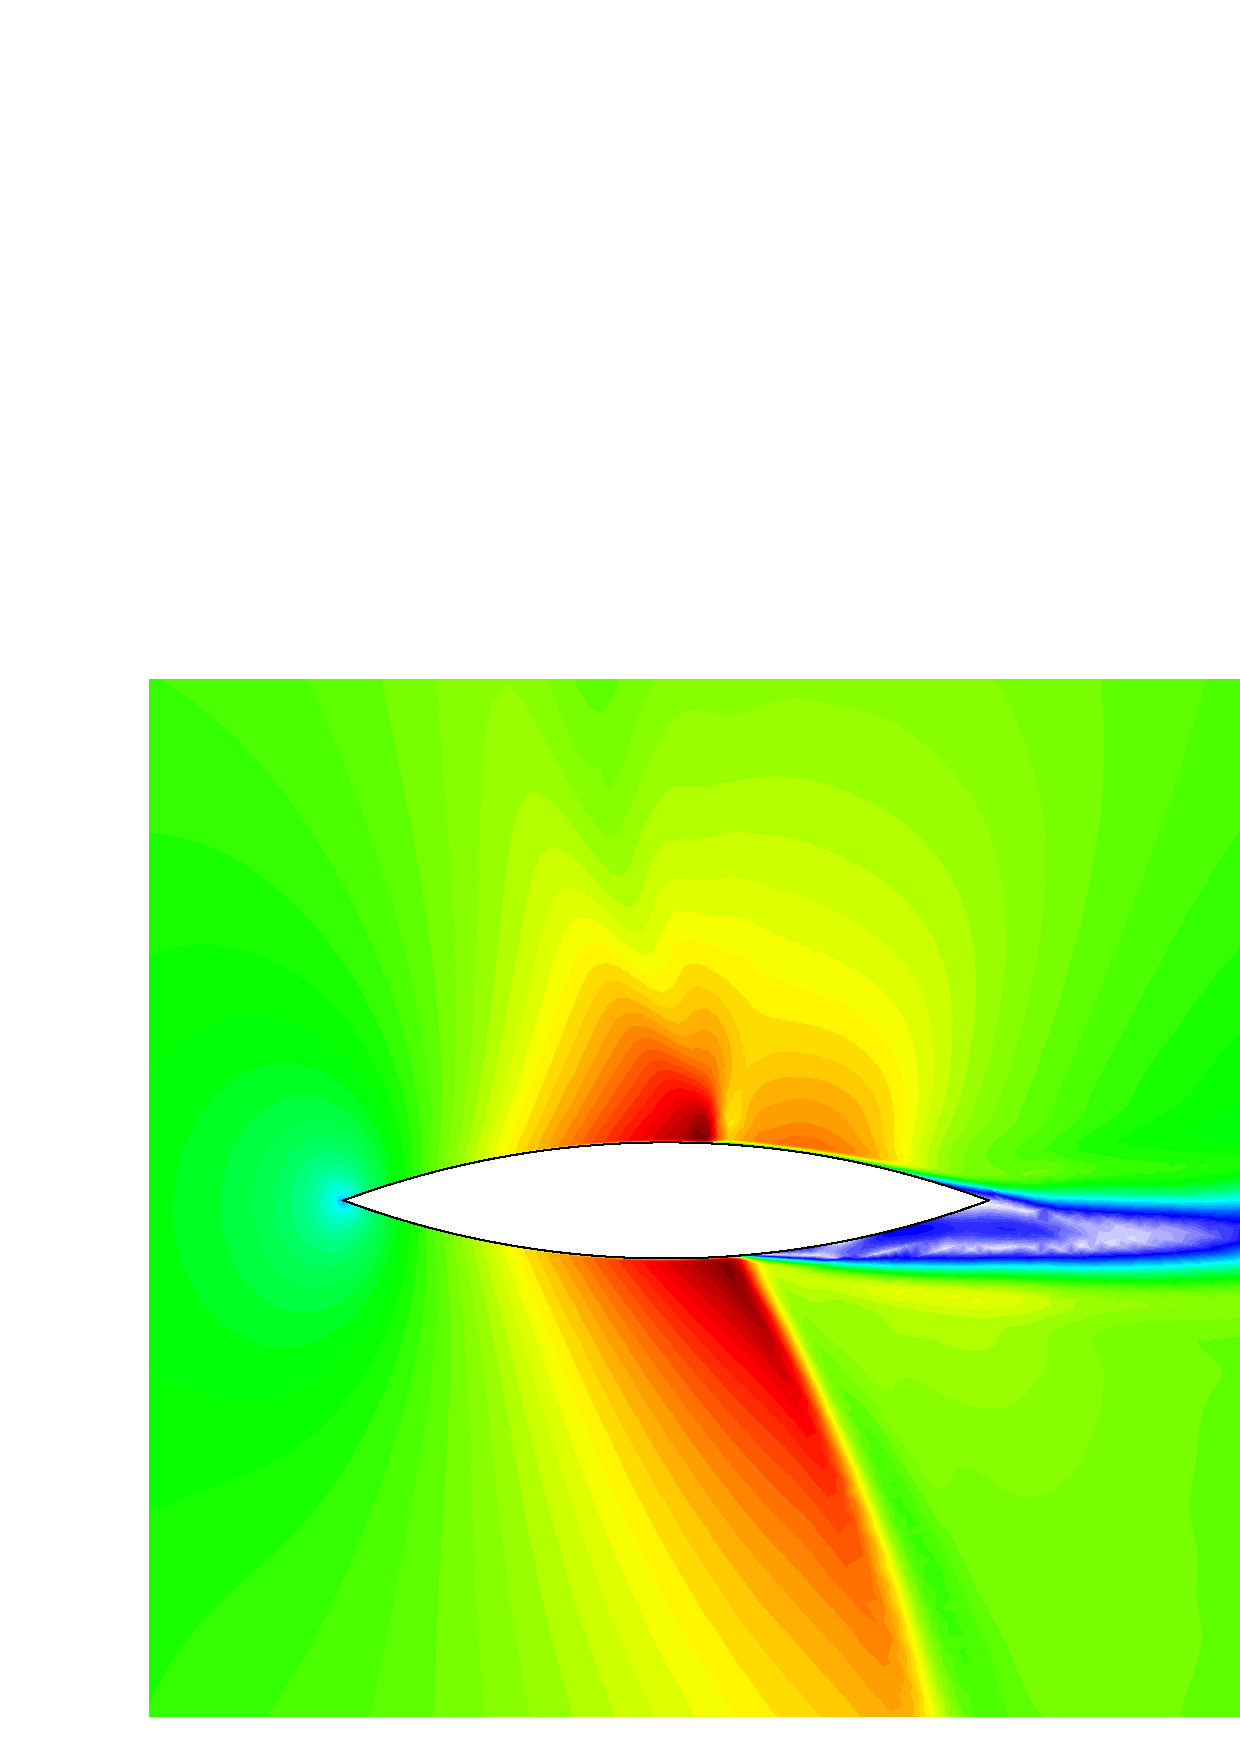
\includegraphics[width=45mm,clip=t]{CHAP_NONLIN/FIGURE/arc11.pdf}}
        &
    \subfigure
       {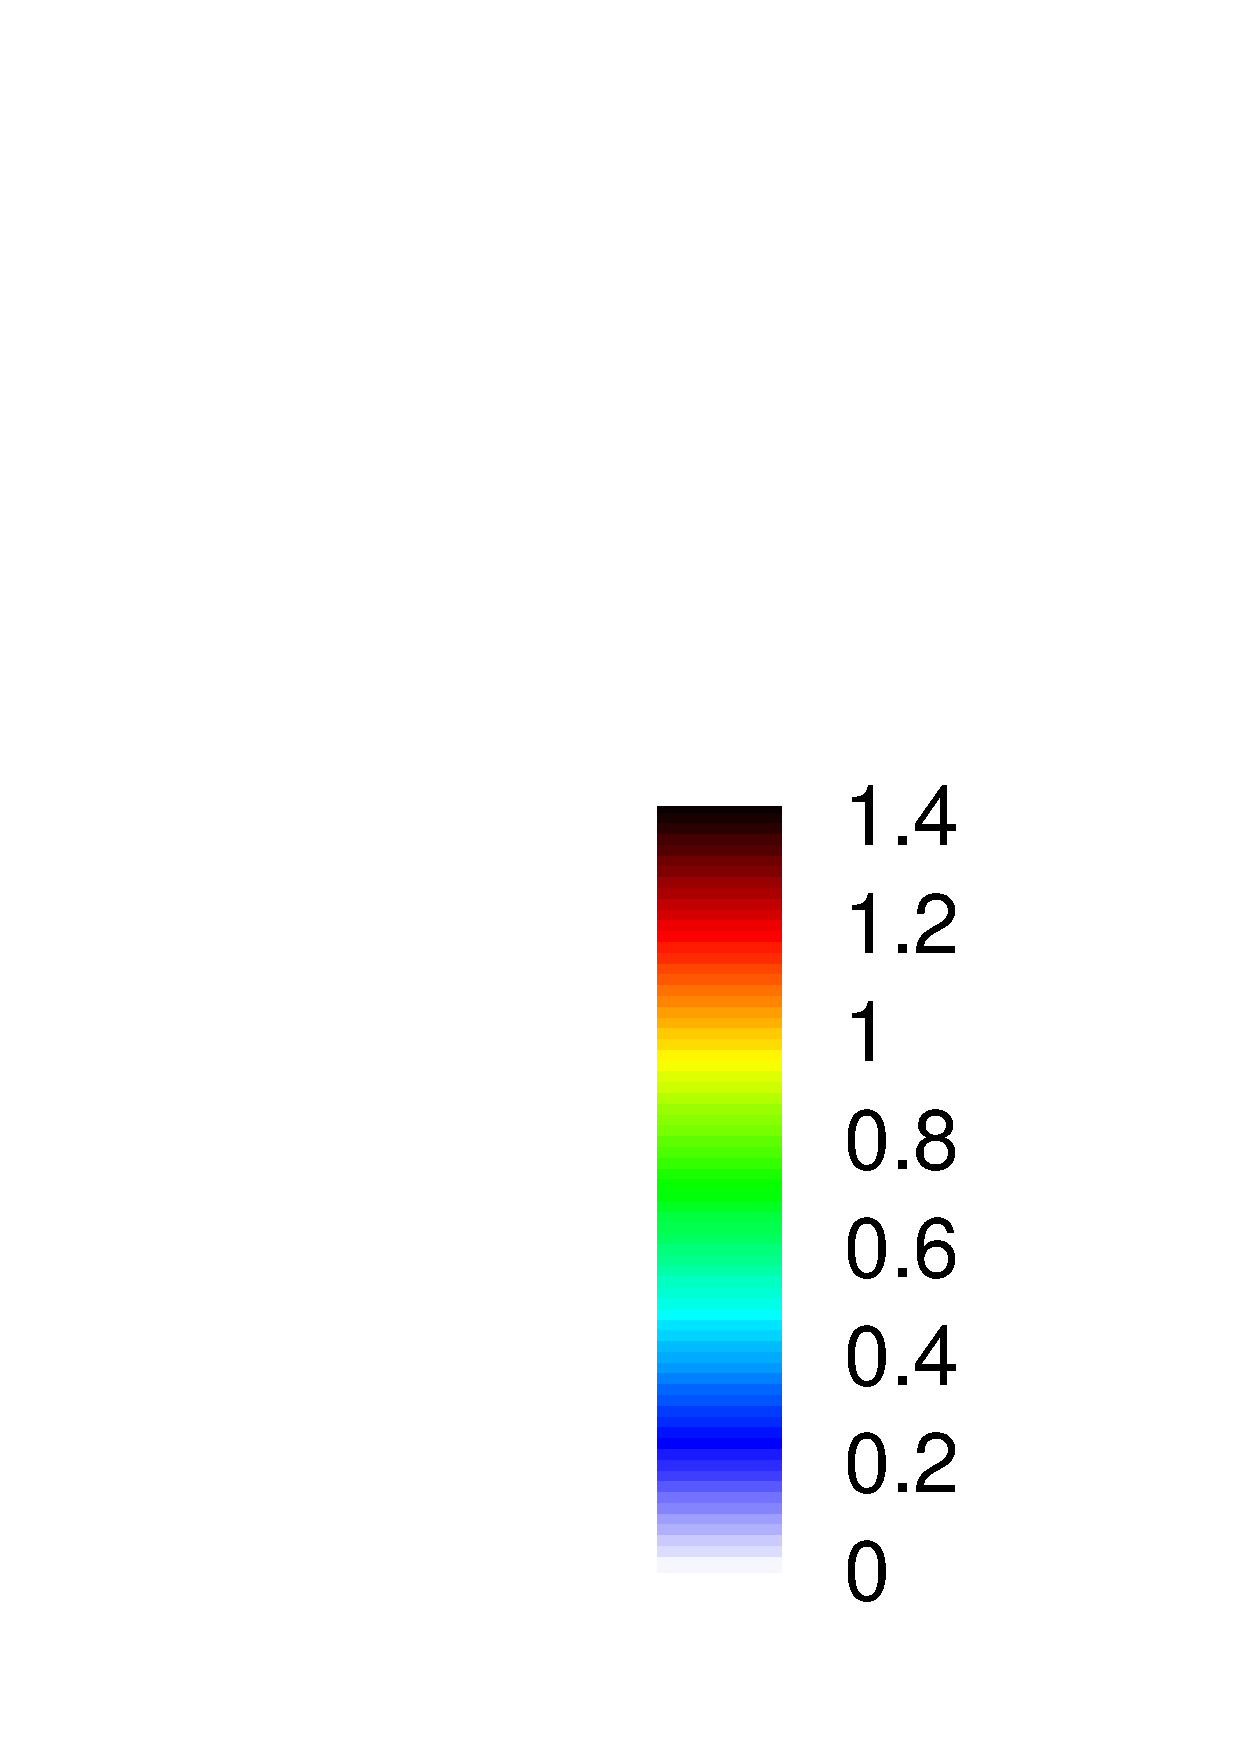
\includegraphics[width=45mm,clip=t]{CHAP_NONLIN/FIGURE/arc12.pdf}}
  \end{tabular}
 \end{center}
 \vspace{-5mm}
 \caption{Bicircular airfoil. $M_\infty = 0.775$,
          $Re_\infty = 7\cdot10\se{6}$. Instantaneous Mach number contours}
 \label{arc_sol1.fig}
\end{figure}
%
 At a free-stream Reynolds number of 7 million, experiments suggest
 transonic buffeting at a free stream Mach number in the range
 from 0.76 to 0.78. On the contrary, the calculations show
 unsteadiness in the Mach number range from 0.765 up to 0.83.
 The computed buffeting reduced frequency $\pi f c/u\sm{\infty}$
 matches the experimental one of $\approx 0.5$.

 Fig. \ref{arc_sol1.fig} reports instantaneous Mach number contours
 in eleven instants over a cycle while Fig. \ref{arc_sol2.fig}a
 shows the average and range of pressure coefficient distribution
 in the airfoil surface.
%
\begin{figure}
 \begin{center}
  \begin{tabular}{c}
    \subfigure[pressure coefficient distribution]
     {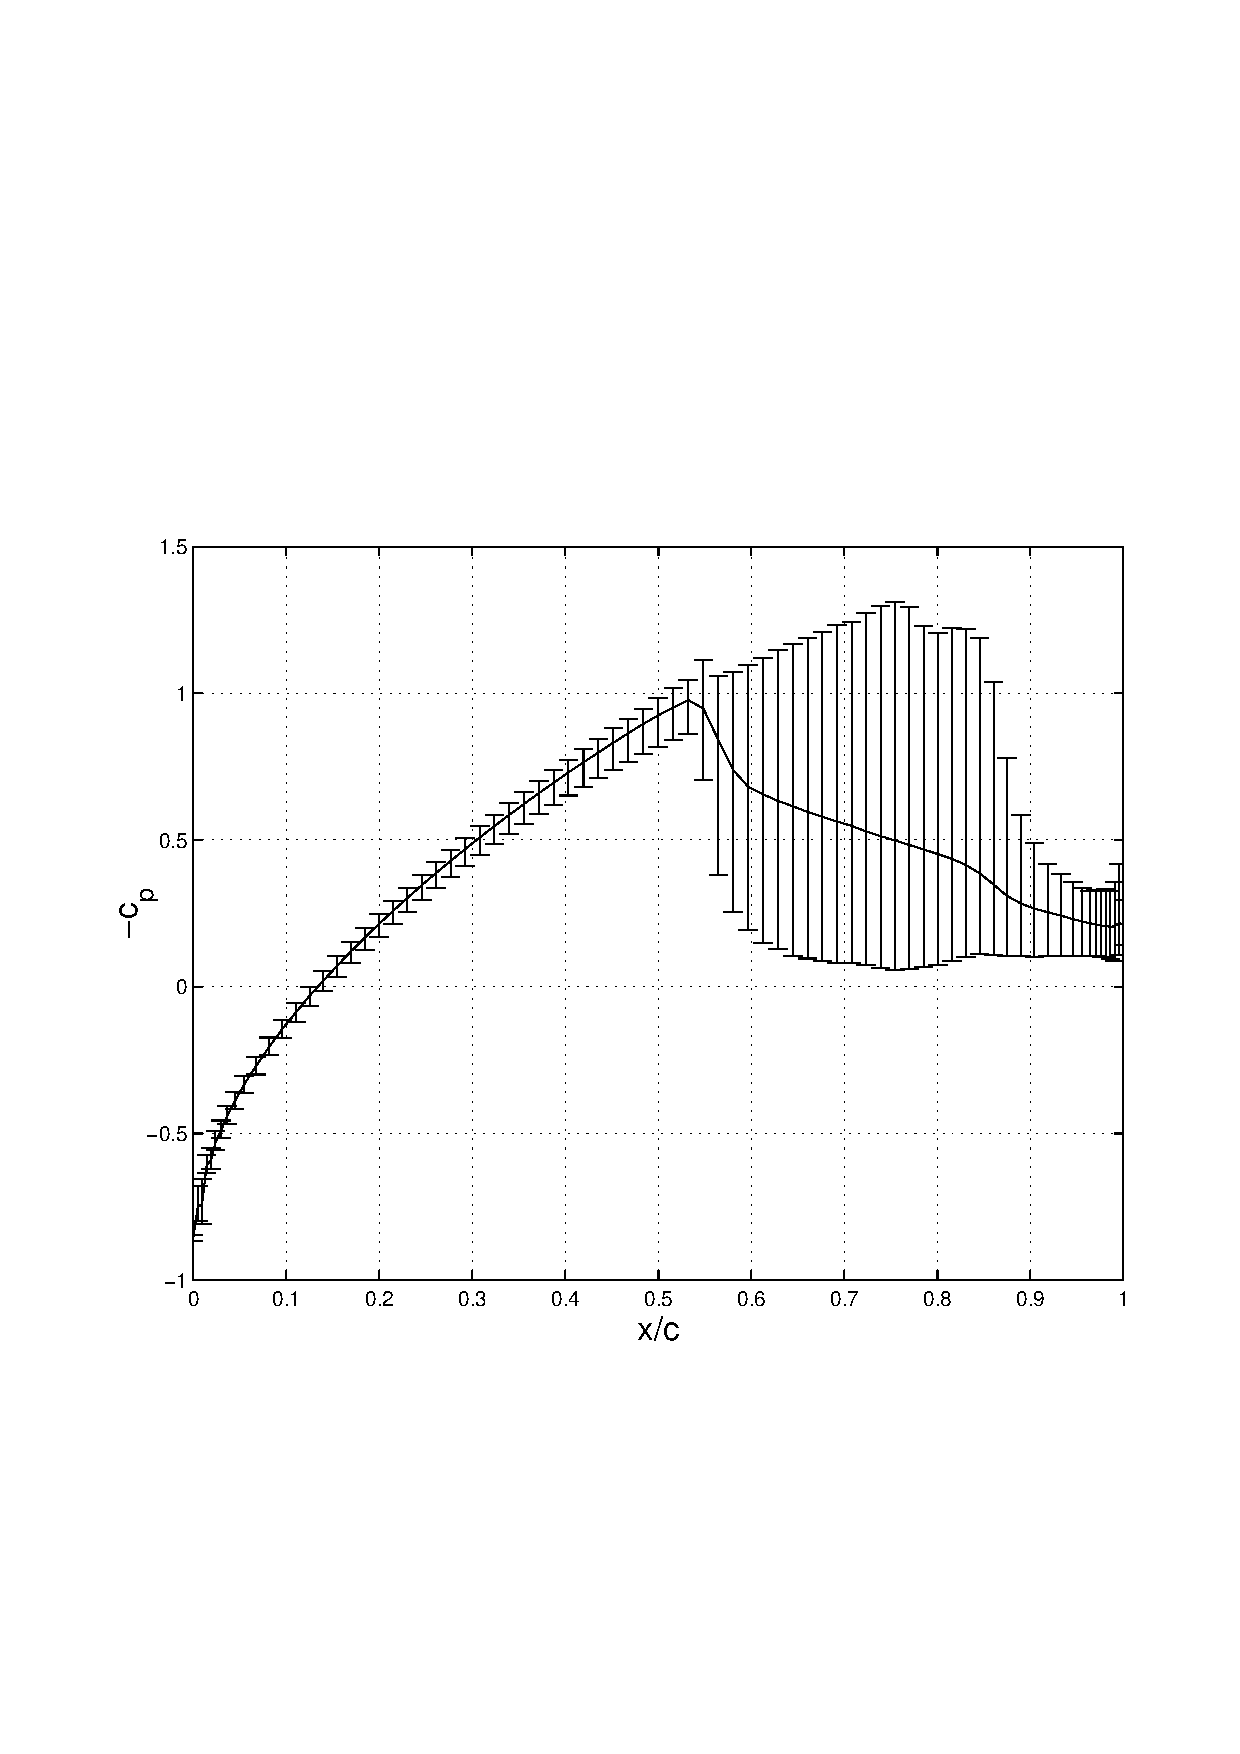
\includegraphics[height=90mm,clip=t]{CHAP_NONLIN/FIGURE/arc_uns.pdf}}
        \\
    \subfigure[pressure coefficient evolution]
     {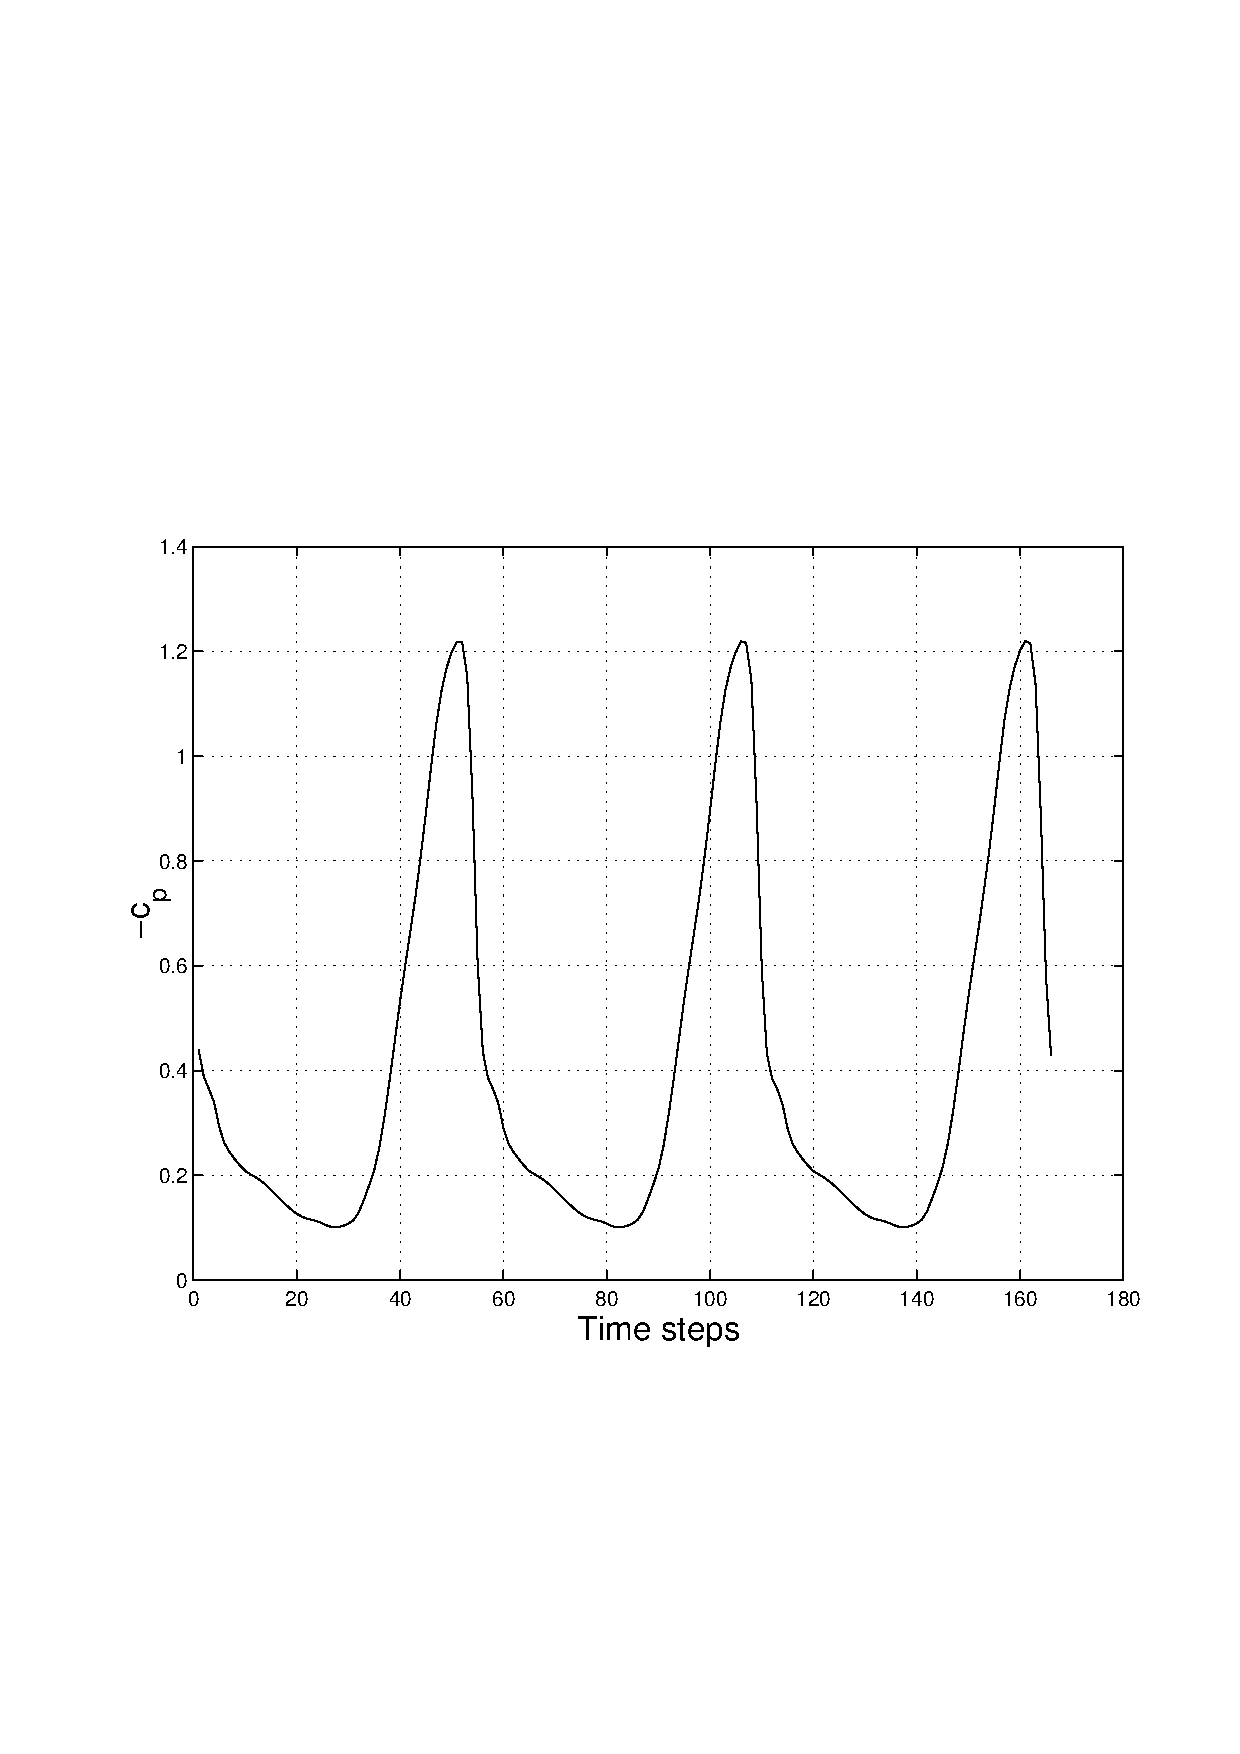
\includegraphics[height=90mm,clip=t]{CHAP_NONLIN/FIGURE/arc_per.pdf}}
  \end{tabular}
 \end{center}
 \vspace{-5mm}
 \caption{Bicircular airfoil. Computed pressure coefficient}
 \label{arc_sol2.fig}
\end{figure}
%
 Fig. \ref{arc_sol2.fig}b reports the evolution in time of the pressure
 coefficient at a point in the airfoil corresponding to $x/c = 0.7$.
 The time history refers to three cycles of oscillation after a periodic
 flow  condition is reached. The calculations were performed
 using roughly 45 divisions over a cycle
 (as indicated in Fig. \ref{arc_sol2.fig}b). This correspond to a local CFL
 number between 0.1 in the far-field and 10,000 in the boundary layer.
%
%
